%%%%%%%%%%%%%%%%%%%%%%%%%%%%%%%%%%%%%%%%%%%%%%%%%%%%%%%%%%%%%%%%%%%%%%%%%%%%%%%%%%%%%%%%%%%%%%%%%%%
%%%%%%%%%%%%%%%%%%%%%%%%%%%%%%%%%%%%%%%%%%%%%%%%%%%%%%%%%%%%%%%%%%%%%%%%%%%%%%%%%%%%%%%%%%%%%%%%%%%
%%%%%%%%%%%%%%%%%%%%%%%%%%%%%%%%%%%%%%%%%%%%%%%%%%%%%%%%%%%%%%%%%%%%%%%%%%%%%%%%%%%%%%%%%%%%%%%%%%%

\chapter{Marco conceptual del problema}

Para poder identificar marcadores significativos para el diagnóstico del deterioro cognitivo, es 
posible usar la técnica de electroencefalografía, que es usada para medir cierto tipo de actividad 
cerebral y que posiblemente esté asociada al deterioro cognitivo. 
%
En esta sección se presenta el deterioro cognitivo en adultos mayores, con énfasis en su 
caracterización.

%%%%%%%%%%%%%%%%%%%%%%%%%%%%%%%%%%%%%%%%%%%%%%%%%%%%%%%%%%%%%%%%%%%%%%%%%%%%%%%%%%%%%%%%%%%%%%%%%%%
%%%%%%%%%%%%%%%%%%%%%%%%%%%%%%%%%%%%%%%%%%%%%%%%%%%%%%%%%%%%%%%%%%%%%%%%%%%%%%%%%%%%%%%%%%%%%%%%%%%

\section{Psicología}

La \textbf{demencia} es, según el Manual diagnóstico y estadístico de trastornos mentales, en su 
quinta versión (DSM-V, por sus siglas en inglés)
\begin{quote}
Un síndrome que consiste en el desarrollo de déficit cognoscitivos suficientemente graves como para 
interferir significativamente en las actividades laborales y sociales, respecto al nivel de 
actividad previo \cite{DCM5}.
%
Los sujetos con demencia tienen una baja capacidad para aprender información nueva y suelen olvidar 
lo aprendido anteriormente, siendo éste el síntoma más prominente.
\end{quote}

Cuando un sujeto presenta cambios marcados en su conducta, es relativamente fácil identificar la 
demencia; caso contrario es el diagnóstico temprano de la misma, el cual es importante para un 
tratamiento adecuado que revierta o desacelere el avance de este síndrome \cite{Knopman01}.

Considerando a los \textbf{adultos mayores} --entendidos como individuos de 60 años o más--
conviene mencionar que el envejecimiento es determinado por una serie de procesos moleculares, 
celulares, fisiológicos y psicológicos que conducen directamente al deterioro de funciones 
cognitivas, específicamente atención y memoria \cite{Park09}.
%
La funcionalidad durante esta etapa se relaciona con el estilo de vida, los factores de riesgo, el 
acceso a la educación y las acciones para el cuidado de la salud realizadas en edades más 
tempranas \cite{Sanhueza14}.

Al momento de diagnosticar deterioro cognitivo en adultos mayores, deben tenerse en cuenta el 
envejecimiento normal y la posible \textbf{pseudodemencia depresiva}, ya que presentan 
características similares. 
%
Con respecto a ésta última, definida como \textit{un trastorno del afecto y que produce un aparente 
deterioro cognitivo} \cite{DCM5}, aunque no se suele considerar como un tipo de demencia.

Así mismo, para realizar un diagnóstico temprano se considerará como etapa precursora de la 
demencia al \textbf{deterioro cognitivo leve}, definido como 
\begin{quote}
Una alteración adquirida y prolongada de una o varias funciones cognitivas, que no corresponde a un 
síndrome focal y no cumple criterios suficientes de gravedad para ser calificada como demencia
\cite{Robles02}.
\end{quote}
dentro del presente escrito, este síndrome será manejado como \textbf{posible deterioro cognitivo} 
(PDC) amén de que está etapa de daño se considera reversible.

%%%%%%%%%%%%%%%%%%%%%%%%%%%%%%%%%%%%%%%%%%%%%%%%%%%%%%%%%%%%%%%%%%%%%%%%%%%%%%%%%%%%%%%%%%%%%%%%%%%
%%%%%%%%%%%%%%%%%%%%%%%%%%%%%%%%%%%%%%%%%%%%%%%%%%%%%%%%%%%%%%%%%%%%%%%%%%%%%%%%%%%%%%%%%%%%%%%%%%%

\subsection{Psicometría}

En psicología los instrumentos de medición comunes son las \textbf{pruebas neuropsicológicas}, 
entendidas como muestras de alguna conducta de interés a las que se asignan puntajes para comparar 
cuantitativamente a los sujetos \cite{Ardila12}.
%
Es a través de estas herramientas que se declaran formalmente las deficiencias cognitivas o 
conductuales, así como su severidad y clasificación.

Las habilidades que se miden usando este tipo de pruebas se suelen agrupar en áreas o 
\textbf{dominios}: atención, lenguaje, cálculo, memoria y aprendizaje, percepción, motricidad, 
funciones somatosensoriales, habilidades espaciales, funciones ejecutivas, entre otros. 
%
La clasificación de dominios suele variar según algunos autores.

En el estudio realizado por Vázquez-Tagle en 2016 \cite{VazquezTagle16} se investigó el deterioro
cognitivo en el estado de Hidalgo, para lo cual se aplicó la siguiente batería de pruebas
neuropsicológicas:
\begin{itemize}
\item Estado cognoscitivo general
\begin{itemize}
\item {Evaluación Neuropsicológica (\textbf{Neuropsi})} \cite{Solis03}
\item {Mini Mental State Examination (\textbf{MMSE})} \cite{Velasco15}
\end{itemize}
\item Detectar pseudodemencia depresiva y ansiedad
\begin{itemize}
\item {Escala breve para la detección de ansiedad del anciano (\textbf{SATS})} \cite{Vargas11}
\item {Escala de Depresión Geriátrica (\textbf{GDS})} \cite{Yesavage82,Greenberg12}
\end{itemize}
\item Detectar cambios en la vida cotidiana
\begin{itemize}
\item {Escala sobre las actividades cotidianas de la vida diaria (\textbf{KATZ})} \cite{Roumec14}
\end{itemize}
\end{itemize}

%%%%%%%%%%%%%%%%%%%%%%%%%%%%%%%%%%%%%%%%%%%%%%%%%%%%%%%%%%%%%%%%%%%%%%%%%%%%%%%%%%%%%%%%%%%%%%%%%%%
%%%%%%%%%%%%%%%%%%%%%%%%%%%%%%%%%%%%%%%%%%%%%%%%%%%%%%%%%%%%%%%%%%%%%%%%%%%%%%%%%%%%%%%%%%%%%%%%%%%

\section{Fisiología}

El registro de la actividad eléctrica en el cerebro, referido como \textbf{electroencefalograma} 
(EEG), está tradicionalmente relacionado con la exploración de procesos mentales y sus trastornos; 
como ejemplo se puede citar que Hans Berger, reconocido como el inventor del EEG, reportó usar 
dicha técnica en 1932 para estudiar posibles cambios en un paciente con Alzheimer 
\cite{historia_eeg}.

El mecanismo base para la propagación de campos eléctricos en las neuronas, depende de la 
capacidad de la membrana celular para mantener un equilibrio estable de iones con el medio 
extracelular.
%
Dicho fenómeno fue ampliamente estudiado por Hodgkin y Huxley y puede describirse brevemente de la 
siguiente manera: cuando existe un desequilibrio puntual y súbito en la concentración extracelular 
de iones, se bombean iones a través de la membrana para restablecer el equilibrio en tal punto; 
esta acción genera desequilibrios secundarios en regiones vecinas de la membrana, que a su vez 
activan mecanismos similares. 
%
Como consecuencia, la perturbación en el potencial de membrana se propaga a lo largo de ésta y se 
genera la transmisión de impulsos nerviosos en neuronas.
%
Un excelente referente sobre el tema es el libro por Ermentrout \cite{Ermentrout10}.

El EEG mide indirectamente la transmisión de impulsos nerviosos entre neuronas de la corteza 
cerebral, de modo que constituye una medida del la \textit{cantidad} de actividad cerebral. 
%
La actividad registrada en el EEG consta principalmente de la actividad postsináptica de las 
neuronas piramidales en la corteza cerebral; éstas se encuentran altamente conectadas entre sí y
forman capas densas.

%%%%%%%%%%%%%%%%%%%%%%%%%%%%%%%%%%%%%%%%%%%%%%%%%%%%%%%%%%%%%%%%%%%%%%%%%%%%%%%%%%%%%%%%%%%%%%%%%%%
%%%%%%%%%%%%%%%%%%%%%%%%%%%%%%%%%%%%%%%%%%%%%%%%%%%%%%%%%%%%%%%%%%%%%%%%%%%%%%%%%%%%%%%%%%%%%%%%%%%

\subsection{Polisomnografía}

Usualmente estos registros de EEG muestran una actividad oscilatoria continua y cambiante, cuya
frecuencia se considera entre 0.5 y 100 \hz. Su composición está fuertemente relacionada con el 
grado de actividad mental mostrando diferencias claras durante vigilia y sueño, o durante quietud 
y concentración \cite{Clark98_2}.

Aunque el EEG es irregular la mayor parte del tiempo, también muestran patrones relativamente 
organizados conocidos como \textbf{ondas cerebrales}. 
%
Las ondas cerebrales más comunes y estudiadas se tipifican en cuatro grupos según su 
\textit{frecuencia}: alfa, beta, gamma, delta, theta.
%
En la figura \ref{ritmos} se representa un arquetipo visual de cada tipo de onda.

\begin{figure}
\centering
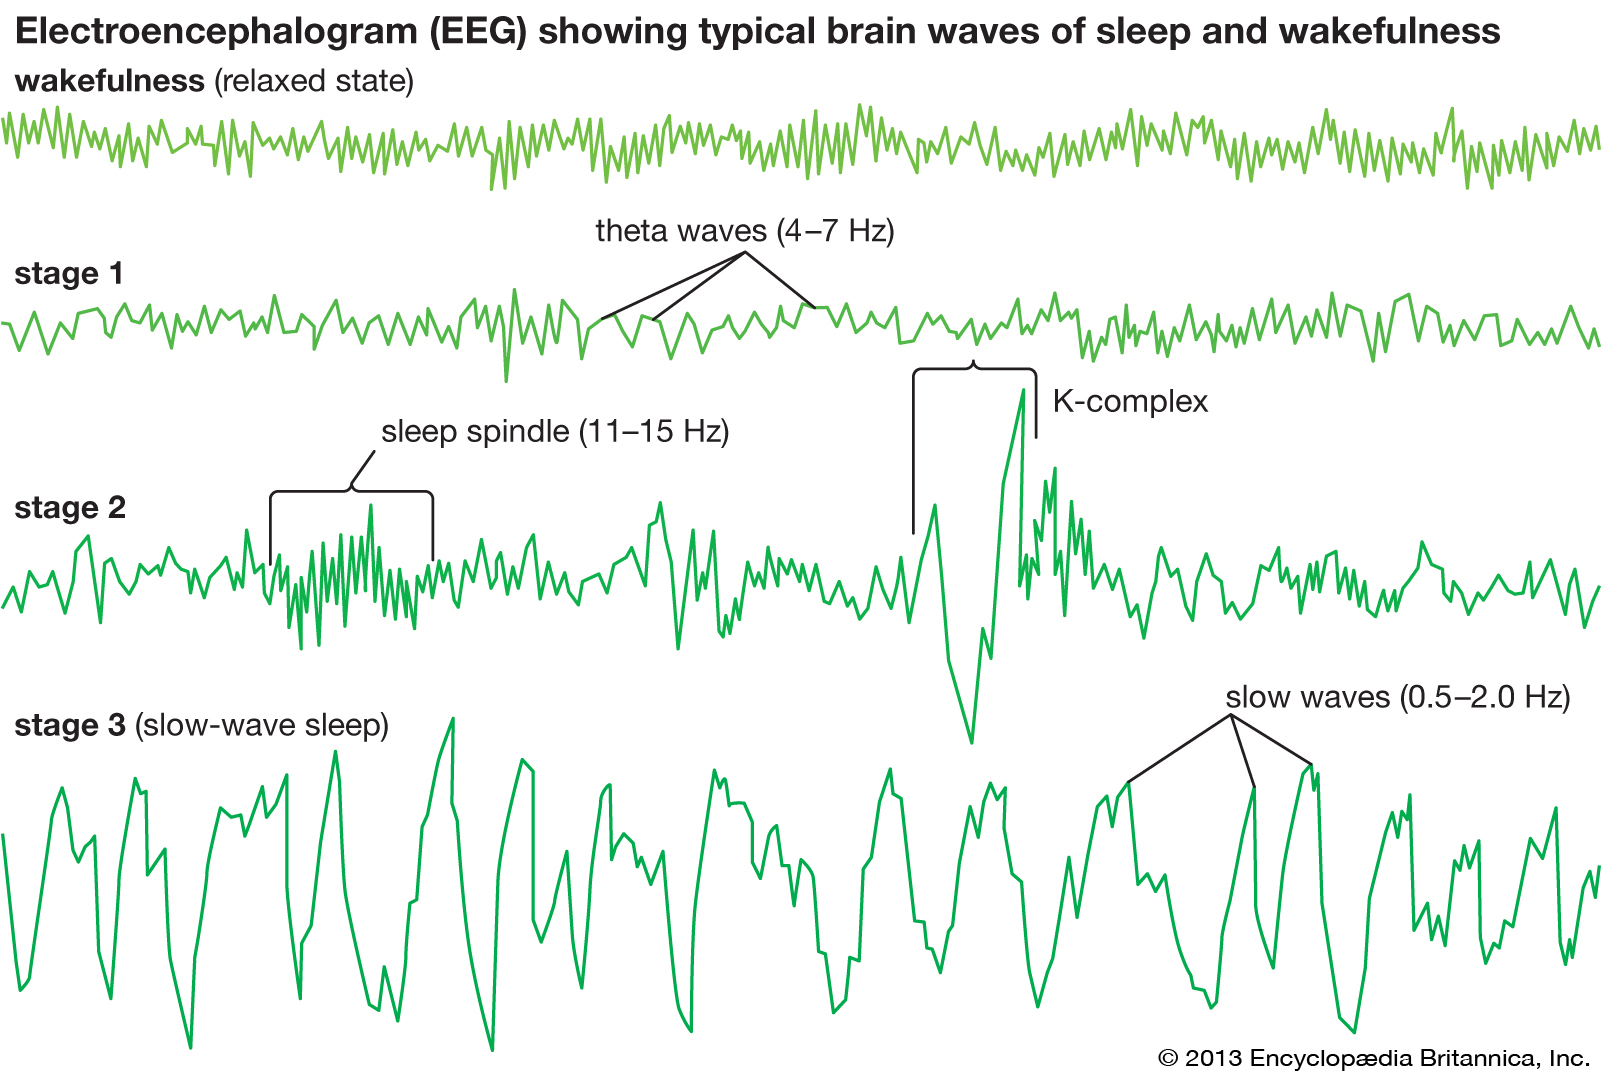
\includegraphics[width=0.95\linewidth]{./img_diagramas/ondas_britannica.jpg} 
\caption[Ejemplos de ondas cerebrales encontradas en el EEG]
{Ejemplos de ondas cerebrales encontradas en el EEG. Imagen tomada de Encyclop{\ae}dia Britannica, 
versión en línea \cite{Britannica}.}
\label{ritmos}
\end{figure}

\begin{table}
\centering
\caption{Generalidades sobre ondas cerebrales}
{\small
\begin{tabular}{lclll}
\toprule
Tipo de onda & Frecuencia [\hz] & {Ubicación usual} & {Condiciones usuales} \\
\midrule
Delta & 0.5 -- 3.5 &         & Síndromes focales. Sueño \\
      &            &         & profundo en infantes \\
Theta & 3.5 -- 7   & P, T    & Durante estrés emocional \\
      &            &         & En infantes \\
Alfa  & 7 -- 12    & F, P, O & Vigilia en reposo con \\
      &            &         & ojos cerrados \\
Beta  & 12 -- 30   & P, F    &      Actividad mental en\\
      &            &         & adultos \\
Gamma & 30 -- 100  &         &\\
      &            &         & \\
%\midrule
%{Husos de} &&&\\
%sueño &&& \\
%{Complejo K} &&&\\
%&&& \\
\bottomrule
\end{tabular}\\
Se abrevian los lóbulos cerebrales: F=frontal, P=parietal, T=temporal, O=occipital.
}
\label{tabla_ondas}
\end{table}

Para realizar el registro \textit{per se} en una forma estandarizada y comparable, se definen
arreglos llamados \textbf{montajes}, entendidos como el conjunto de (1) los sitios donde se colocan 
los electrodos de registro y (2) la manera en que los electrodos de registro están conectados entre 
sí.

En el trabajo de Vázquez Tagle \cite{VazquezTagle16} se usa un montaje \textit{referencial}, en el 
cual los electrodos se conectan en paralelo con un electrodo de referencia cuya actividad eléctrica 
es constante y negligible (lóbulos de las orejas, electrodos cortocircuitados A1, A2); los 
electrodos fueron colocados según el \textbf{Sistema 10--20} \cite{Jasper58,Klem99}.
%
Dicho sistema define los sitios según una cuadrícula construida respecto a distancias relativas 
entre varios puntos de referencia: el \textit{inion}, protuberancia en la región posterior del 
cráneo, el \textit{nasión}, unión del hueso frontal y los huesos nasales, y el \textit{punto 
preauricular}, ubicado arriba del cartílago que protege el canal auditivo.

\begin{figure}
\centering
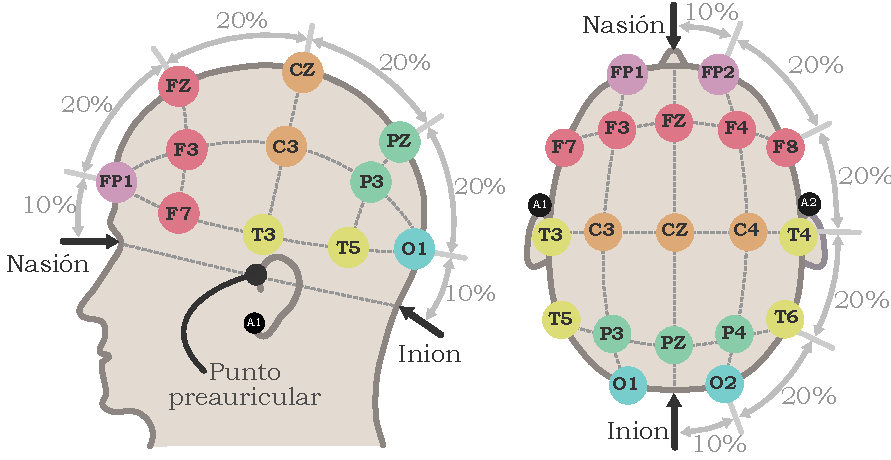
\includegraphics[width=\linewidth]{./img_diagramas/cabeza_proporcionada_color_v4.pdf} 
\caption{Colocación de electrodos según el sistema 10--20}
\label{img1020}
\end{figure}

Debido a que las neuronas en la corteza cerebral tienen orientaciones muy diversas y a que disparan 
de manera asíncrona, además de que el cerebro se encuentra cubierto por las muchas capas descritas
anteriormente, las señales captadas por los electrodos deben ser amplificadas analógicamente antes 
de ser registradas digitalmente.
%
A ello hay que añadir la difusión generada por las meninges, el líquido encefalorraquídeo y el 
cráneo.

Un efecto colateral de amplificar la señal es la inclusión de \textbf{ruido}, entendido como 
señales que son registradas de manera no deseada; como ejemplo, los músculos faciales medianamente 
contraídos generan campos eléctricos con frecuencia de 100 \hz.
%
Este tipo de ruido \textit{persistentes} son eliminados usando un filtro que \textit{elimine} los 
componentes de frecuencia específicos.
%
Los ruidos de duración corta son referidos como \textbf{artefactos}; como ejemplo, pestañear 
voluntariamente durante un episodio de quietud mental interrumpe las ondas alfa por cerca de dos 
segundos. 

Adicionalmente al registro del EEG, la PSG contempla el registro de algunas otras \textit{variables 
fisiológicas} como respiración, ritmo cardíaco, temperatura, entre otros. 
%
En el estudio por Vázquez Tagle y colaboradores, el registro de PSG incluyó registros de actividad 
ocular (\textbf{electrooculograma}, EOG) y tono muscular (\textbf{electromiograma}, EMG), según las 
recomendaciones de la AASM para clasificar las etapas de sueños. La ubicación estos últimos 
electrodos es ilustrada en la figura \ref{emg_eog}.

\begin{figure}
\centering
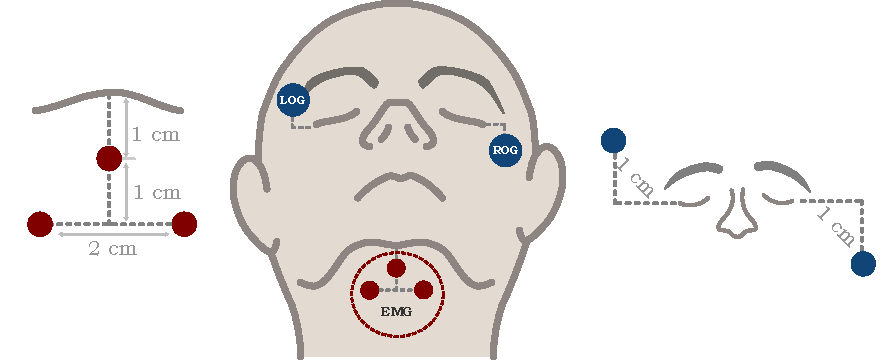
\includegraphics[width=\linewidth]
{./img_diagramas/emg_eog_v4.pdf}
\caption{Colocación de electrodos para registrar actividad ocular y tono muscular}
\label{emg_eog}
\end{figure}

Para interpretar los registros de EOG (canales LOG, ROG) se puede entender al ojo como una batería
cuyos  polos son la retina y la pupila, y que genera pequeñas variaciones en el campo eléctrico
cuando se mueve; el registro consiste en la proyección del movimiento sobre el eje que forman los
electrodos.
%
Los registros de EMG (canal EMG) admiten una interpretación más \textit{sencilla}, ya que los
músculos son activados directamente por señales eléctricas: el tono muscular es la actividad 
muscular basal, y se relaciona con la velocidad con que los músculos pueden \textit{salir} del 
reposo.

%%%%%%%%%%%%%%%%%%%%%%%%%%%%%%%%%%%%%%%%%%%%%%%%%%%%%%%%%%%%%%%%%%%%%%%%%%%%%%%%%%%%%%%%%%%%%%%%%%%
%%%%%%%%%%%%%%%%%%%%%%%%%%%%%%%%%%%%%%%%%%%%%%%%%%%%%%%%%%%%%%%%%%%%%%%%%%%%%%%%%%%%%%%%%%%%%%%%%%%

\subsection{Estructura del sueño}

Se entiende al sueño como un proceso vital, con una estructura característica, y que en el ser 
humano presenta las siguientes propiedades \cite{CarrilloMora}:
\begin{enumerate}
\item Disminución de conciencia y reactividad a estímulos externos
\item Fácilmente reversible, a diferencia de estados patológicos como estupor y coma
\item Inmovilidad y relajación muscular
\item Periodicidad típica circadiana (diaria)
\item Los individuos adquieren una postura estereotipada
\item La privación induce alteraciones conductuales y 
fisiológicas, además de que genera una \textit{deuda} acumulativa
\end{enumerate}

La duración del sueño es determinada en gran parte por la edad; el recién nacido duerme entre 14 y 
18 horas, el lactante entre 12 y 14 horas, el niño en etapa escolar entre 11 y 12 horas y en la 
edad adulta, la mayoría duerme entre 7 y 8 horas por noche \cite{Contreras13}.
%
Paralelamente el sueño no es un proceso homogéneo, sino que tiene una estructura por etapas con 
rasgos electroencefalográficos y fisiológicos distintivos.

Para su estudio, el sueño se divide en dos etapas: N y R.
%
La \textbf{fase N}, se caracteriza por movimientos oculares lentos, tono muscular que decrece 
constantemente, actividad cerebral que recuerda al reposo, y la presencia de husos de sueño y 
complejos K; en base a ello se divide en las sub-fases N1, N2, N3.

Durante la \textbf{fase R} el tono muscular disminuye (excepto para los músculos respiratorios y 
los esfínteres), la frecuencia cardíaca y respiratoria se vuelve irregular, y el sujeto exhibe 
movimientos oculares rápidos (MOR); en base a lo cual la fase R es conocida como \textbf{sueño 
MOR}.
%
En el EEG, aparecen ondas rápidas de bajo voltaje, irregulares, y que recuerdan la actividad 
durante el estado de alerta; estos patrones no interrumpen el sueño sino que, contrariamente,
incrementan el umbral para estímulos externos, motivo por el cual esta fase también es referida 
como \textbf{sueño paradójico}.
%
Cabe mencionar que durante el sueño MOR se producen la mayoría de las ensoñaciones (referidas 
coloquialmente como \textit{sueños}), y que la mayoría de los pacientes que despiertan durante esta 
fase suelen recordar vívidamente el contenido de sus ensoñaciones \cite{Rosales14}.

\begin{table}
\caption[Criterios para la clasificación de etapas de sueño]
{Criterios para la clasificación de etapas de sueño según la AASM}
\centering
{\small
\begin{tabular}{lllll}
\toprule
&&   & Movimientos & Tono \\
\multicolumn{2}{l}{Etapa}& Características del EEG & oculares & muscular \\
\midrule
Vigilia & W  & {Ritmo alfa} en $>50$\% de la época en   & No & Alto \\
        &    & la región occipital                &    &      \\
NMOR 1  & N1 & Cambio de alfa por AABFM, atenuación & Lentos & $<$W     \\
        &    & del ritmo dominante. Ondas agudas   &    &      \\
NMOR 2  & N2 & Husos de sueño y complejos K en la    & No & $<$W, $>$R     \\
        &    & primera mitad de la época. AABFM &    &     \\
NMOR 3  & N3 & {Ondas lentas} (0.5--2 \hz, $>75$ \mv) en& No & $<$N2, $\approx$R \\
        &    & $>20$\% de la época. Husos de sueño       &&      \\
MOR     & R  & Actividad baja amplitud y frecuencias & MOR's & Bajo  \\
        &    & mixtas. Ondas 'saw-tooth'             &       &       \\
\bottomrule
\multicolumn{4}{l}{Se abrevia AABFM=Actividad de Amplitud Baja y Frecuencias Mixtas}
\end{tabular}\\
}
\end{table}

\begin{figure}
\centering
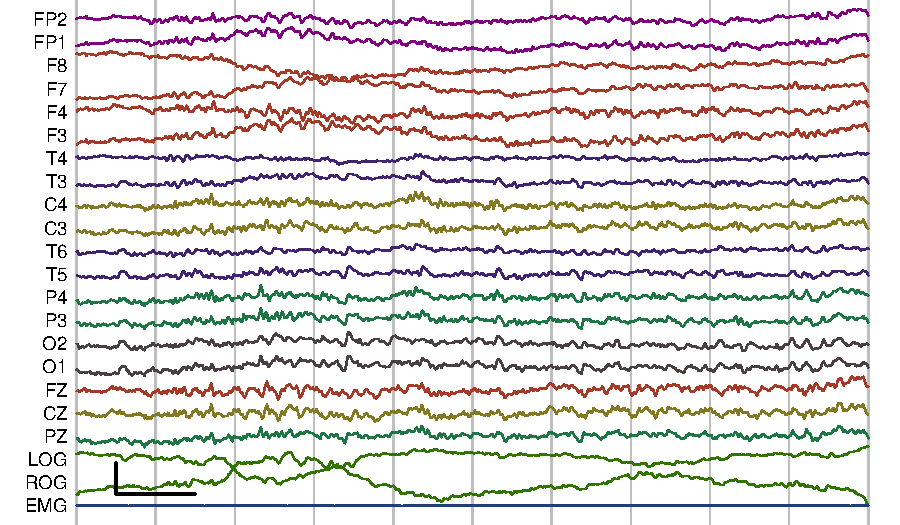
\includegraphics[width=\linewidth]
{./img_ejemplos/MJNN_epoca_stam.pdf}
\caption[Registro de polisomnograma durante sueño MOR]
{Registro de polisomnograma durante sueño MOR. Marca de calibración: vertical, 10 \mv, horizontal, 
1 segundo}
\label{ejemplos_mor}
\end{figure}

%%%%%%%%%%%%%%%%%%%%%%%%%%%%%%%%%%%%%%%%%%%%%%%%%%%%%%%%%%%%%%%%%%%%%%%%%%%%%%%%%%%%%%%%%%%%%%%%%%%
%%%%%%%%%%%%%%%%%%%%%%%%%%%%%%%%%%%%%%%%%%%%%%%%%%%%%%%%%%%%%%%%%%%%%%%%%%%%%%%%%%%%%%%%%%%%%%%%%%%
%%%%%%%%%%%%%%%%%%%%%%%%%%%%%%%%%%%%%%%%%%%%%%%%%%%%%%%%%%%%%%%%%%%%%%%%%%%%%%%%%%%%%%%%%%%%%%%%%%%